\chapter{\IfLanguageName{dutch}{Stand van zaken}{State of the art}}%
\label{ch:stand-van-zaken}

% Tip: Begin elk hoofdstuk met een paragraaf inleiding die beschrijft hoe
% dit hoofdstuk past binnen het geheel van de bachelorproef. Geef in het
% bijzonder aan wat de link is met het vorige en volgende hoofdstuk.

% Pas na deze inleidende paragraaf komt de eerste sectiehoofding.


% TODO: GDPR regulations about storing face data/imgs

\section{Authentication in Digital Security}
Authentication is the process of verifying the identity of users attempting to access digital systems or online services. 
Commonly used methods include knowledge-based authentication (passwords), possession-based methods (tokens), and 
biometric methods like fingerprints and facial recognition \autocite{Pant2022}. Passwords remain dominant due to 
their simplicity and widespread acceptance, but face security issues including password reuse, phishing, and 
brute-force attacks \autocite{Ophoff2021}. For users with cognitive or motor disabilities, these issues are 
further complicated by difficulties in recalling or accurately inputting passwords \autocite{Rochford2014}.

\section{Accessibility Challenges in Authentication}
Individuals with cognitive disabilities, such as memory disorders or conditions like dyslexia, often struggle with remembering complex passwords, resulting in frequent authentication failures and frustration \autocite{Farid2019, Ophoff2021}. Those with motor disabilities, including conditions like Parkinson's disease or cerebral palsy, face physical challenges in typing passwords accurately \autocite{Renaud2020}. The Web Content Accessibility Guidelines (WCAG) highlight the importance of designing authentication systems that minimize these cognitive and physical burdens \autocite{Brewer2023}.

\vspace{4\baselineskip}
\section{Facial Recognition Technology}
Facial recognition works by identifying and verifying individuals from digital images or videos using various algorithmic approaches, including traditional image processing methods and modern deep learning techniques. Notable algorithms include Haar cascades, Eigenfaces, Local Binary Patterns Histograms (LBPH), and Convolutional Neural Networks (CNNs) \autocite{ElSayed2015}. The evolution of deep learning, particularly CNN-based approaches, has significantly enhanced accuracy and reliability, making facial recognition robust even under challenging conditions like variations in lighting, angle, or facial expressions \autocite{ZhangDlib2020}.

\section{Face Recognition as a Biometric Solution}
Biometric authentication, particularly facial recognition, is gaining popularity as it significantly reduces the cognitive and physical effort required by traditional password-based methods \autocite{Furnell2022}. 
Unlike passwords, biometric data are unique physical attributes of an individual, providing an inherent security advantage by eliminating risks associated with knowledge-based authentication methods, 
such as forgetting or sharing passwords \autocite{Pant2022}.

Facial recognition stands out as particularly promising because it is intuitive, does not require manual input, and can be seamlessly integrated into daily digital interactions \autocite{Bhatt2011}. However, biometric systems are not without limitations. Spoofing attacks, privacy concerns, and the requirement for consistent lighting and camera quality present technical and ethical considerations that must be carefully managed \autocite{Kuznetsov2024, Bahia2024}.


\subsection{Comparison of Facial Recognition Libraries}

\subsubsection{OpenCV (Java)}
OpenCV is a widely used open-source library offering classical computer vision techniques such as Haar cascades and LBPH. While effective in controlled environments, it typically requires server-side or desktop-based implementations, limiting its applicability for client-side web applications \autocite{Dominguez2017}.

\subsubsection{face\_recognition in Python}  
The face\_recognition library, built on dlib, is renowned for its accuracy and pre-trained deep learning models. \textcite{ZhangDlib2020} highlight that it excels in applications requiring precision, utilizing techniques like CNN-based face encodings for high-quality results. However, its reliance on Python and backend processing makes it less suitable for client-side, browser-based implementations like those required in this project.

\subsubsection{face-api.js (JavaScript)}
face-api.js, built on TensorFlow.js, runs entirely in the browser, providing a privacy-centric, client-side solution suitable for real-time applications \autocite{Vageele2024}. Its key benefits include privacy (no server-side data transfer), compatibility with modern web frameworks, and modularity for lightweight and efficient real-time processing. These features align closely with the project's emphasis on usability, accessibility, and security, making face-api.js the optimal choice for this research.

\section{Security Considerations for Biometric Authentication}
While facial recognition enhances accessibility, it also introduces specific security concerns. Common vulnerabilities include spoofing attacks using photos or video recordings and data privacy issues related to biometric data storage \autocite{Bowyer2006, Bahia2024}. Beyond these well-known threats, systems that store facial biometric data face additional sophisticated attack vectors:

\begin{itemize}
\item \textbf{Template Extraction Attacks:} These attacks aim to reconstruct biometric templates from stored embeddings, potentially compromising the entire authentication system. Even when templates are encrypted, side-channel attacks can leak information about the underlying biometric data \autocite{Mai2019, Dong2021}. As demonstrated by \textcite{Mai2019}, deep face templates previously thought to be secure can be reverse-engineered to recover recognizable face images, raising significant privacy concerns. Building on this work, \textcite{Dong2021} showed that high-definition face images can be generated from supposedly secure templates using advanced generative models.

\item \textbf{Model Inversion Attacks:} Adversaries can exploit machine learning models to regenerate facial images from stored embeddings or model parameters, effectively reversing the feature extraction process \autocite{Fredrikson2015, Zhang2020}. \textcite{Fredrikson2015} demonstrated that these attacks can leverage confidence information from ML models to reconstruct training data, while \textcite{Zhang2020} advanced this concept with generative model-inversion attacks against deep neural networks. This poses significant privacy risks as it may allow attackers to recreate recognizable facial images from supposedly secure numerical representations.

\item \textbf{Spoofing Attacks:} Presentation attacks using photos or video recordings of legitimate users to deceive recognition systems \autocite{Kuznetsov2024}.
\end{itemize}

\clearpage

Modern mitigation strategies include:
\begin{itemize}
\item \textbf{Liveness Detection:} Techniques to ensure the presence of a real, live user rather than a static image or video \autocite{Kuznetsov2024}.

\item \textbf{Local Data Processing:} Client-side processing prevents the transmission of sensitive biometric data, enhancing privacy.

\item \textbf{Multi-factor Authentication (MFA):} Combining biometric data with other authentication methods to provide layers of security and protect against vulnerabilities inherent in single-method authentication systems \autocite{Furnell2022}.

\item \textbf{Cancelable Biometrics:} Applying irreversible transformations to biometric templates before storage, allowing for template revocation if compromised. \textcite{Rathgeb2011} provide a comprehensive survey of these techniques, highlighting their importance in protecting biometric data while maintaining authentication accuracy.
\end{itemize}

% \section{Adversary Threat Models in Facial Biometric Authentication}
% Modern facial biometric systems must account for various adversary capabilities and attack vectors. Table 1 summarizes three critical threats and effective mitigation strategies, with references to recent literature and technical reports.

% \begin{table}[htbp]
%   \centering
%   \small
%   \begin{tabular}{|p{3.2cm}|p{6.2cm}|p{5.8cm}|}
%     \hline
%     \textbf{Threat} & \textbf{Description} & \textbf{Mitigation(s)} \\
%     \hline
%     \textbf{Offline Database Theft} & Adversary gains unauthorized access to stored biometric templates or face embeddings (e.g., via a database breach). Stolen biometric data can be misused for identity theft or cross-system fraud, since compromised templates allow attackers to impersonate users or perform cross-matching across different services. (Unlike passwords, biometric traits are permanent, so a leaked template poses a long-term risk to the victim.) & Protect stored templates using strong cryptography and transform-based protections. Encrypt biometric databases at rest so stolen files are unusable, and apply non-invertible, revocable transformations (i.e. **cancelable biometrics**) to the templates. Cancelable biometric schemes store only a transformed version of the face data that cannot be reversed and can be *“revoked”* or replaced if compromised. Additional safeguards include multi-factor authentication - ensuring a biometric alone cannot unlock accounts - and hardware security modules for template storage, which together limit the damage from a stolen biometric database. \\
%     \hline
%     \textbf{Compromised Browser Extension} & A malicious or compromised browser extension (or similar client-side malware) intercepts facial data during capture or transmission. The attacker could tap into the live camera feed or extracted face embeddings and steal or manipulate this data in real time. This essentially creates a man-in-the-middle, allowing replay or injection of captured biometric data to fraudulently authenticate as the victim. *In fact, recent banking malware has been observed recording victims' faces and using AI-generated videos (deepfakes) to bypass facial authentication defenses.* & Isolate and secure the biometric processing on the client side, minimizing the extension's access to sensitive data. For example, perform face recognition in a trusted local environment (using in-browser ML libraries or OS-level APIs) so that raw images/embeddings aren't sent over the network. All communication between the browser and any authentication server should be encrypted end-to-end, preventing eavesdropping or tampering in transit. It's also wise to require explicit user presence or a secondary factor (MFA) before finalizing login. This way, even if an extension is compromised, an attacker cannot stealthily authenticate with stolen biometrics alone. Robust code signing and permission controls on extensions further reduce the risk of compromise. \\
%     \hline
%     \textbf{Shoulder-Surfing} & An attacker observes or records the legitimate user's face during an authentication attempt (e.g., looking over the user's shoulder or using a camera from nearby). By capturing the user's facial input, the adversary can later present a **spoof** - such as a photo, video, or mask of the user's face - to impersonate them. Biometric systems eliminate the need to type passwords (mitigating classic shoulder-surfing of secrets), but without countermeasures they remain vulnerable to replay attacks using captured biometric data. In essence, a clear image or video of the user can be “replayed” to fool a naïve face recognition system. & Deploy anti-spoofing and liveness detection measures to ensure the system is interacting with a live user *in real time* rather than a recording or static image. Effective liveness detection techniques include prompting the user to perform random actions (e.g. blink, turn head) or using 3D/infrared cameras to detect depth and vitality cues, which defeats simple photo or video replays. Advanced deep-learning-based **face anti-spoofing** can automatically classify and reject fake vs. live imagery. Furthermore, requiring user attention or a secondary confirmation (such as a phone notification or a known gesture) can mitigate the risk of covert observation. By combining these defenses - liveness verification and optional multi-factor checks - facial authentication systems become much more resistant to shoulder-surfing and presentation attacks. \\
%     \hline
%   \end{tabular}
%   \caption{Adversary capabilities and example mitigations for facial biometric authentication systems.}
%   \label{tab:threat-model}
% \end{table}


\section{Current Limitations in Password Managers}
Password managers simplify password management by securely storing and auto-filling credentials but commonly rely on a master password, perpetuating cognitive and motor accessibility issues. This approach is problematic for users who struggle with memory recall or precise typing \autocite{IALabs2024}. While MFA offers increased security, it often introduces additional complexity that further burdens users with disabilities. Current systems have limited inclusivity and accessibility, reinforcing the need for more intuitive solutions.

\section{Database Options for Client\textendash Side Password Storage}
\label{sec:db-options}

A password manager must choose a local datastore that balances footprint,
offline capability, security, and future synchronisation needs.  The five
candidates below are summarised with literature references and official
documentation links.

\subsection*{SQLite}
\textcite{Gaffney2022} show that SQLite embeds the entire ACID-compliant
engine in a single file of only a few-hundred-kB, requiring no server
process.  Its dynamic typing allows flexible schemas \autocite{Corovcak2025}.
Because it lacks native user authentication, security depends on OS file
permissions or extensions such as SQLCipher \autocite{Corovcak2025}.
Official documentation confirms the zero-config model and SQL feature set
\autocite{sqlLiteDoc2025}. These traits make SQLite ideal for an offline,
single-device password vault, provided the file is encrypted at rest.

\subsection*{PostgreSQL}
PostgreSQL's client-server design provides robust concurrency and rich SQL
features after 35-years of development \autocite{Gkamas2022}. It provides 
built-in role-based access control and supports TLS to secure data in transit.
However, the community edition lacks native encryption at rest, so administrators 
must rely on the \textit{pgcrypto} extension or file-system encryption 
\autocite{Crunchy2024, PostgreSQL2025}. A local instance typically consumes hundreds of-MB of RAM,
which is heavy for a single-user password vault. Hence PostgreSQL is secure and scalable,
but overkill for a single-user application.

\subsection*{MongoDB}
MongoDB stores JSON-like documents in flexible collections and scales
horizontally \autocite{Miryala2024}.  A \texttt{mongod} process needs 1-2-GB
RAM even for modest use \autocite{Dahunsi2021}.  Community builds provide
authentication and TLS, yet encryption at rest is Enterprise-only
\autocite{PrismaMongoEnc, MongoDB2025}, so disk encryption or field-level
crypto is required.  Misconfiguration has repeatedly exposed databases,
underscoring the need for hardened defaults.  The
server footprint makes MongoDB unsuitable for a secure, single-user password vault.

\subsection*{Couchbase Lite}
Couchbase Lite embeds a document store inside the app and syncs through
Sync Gateway when online \autocite{Pal2016}.  Its metadata inflates on-disk
size versus SQLite, yet runtime demands remain mobile-friendly
\autocite{Gkamas2022}.  The Enterprise build supports 256-bit AES encryption
of the local DB \autocite{CouchbaseEncryption, CouchbaseDoc2025}.  Because it
executes in the app's sandbox, further authentication is handled by the host
application.  These qualities make Couchbase Lite attractive for an
offline-first vault that may later sync across devices.

\subsection*{Firebase Cloud Firestore}
Firestore is a serverless NoSQL service that caches data locally and
synchronises transparently once connectivity returns \autocite{FirebaseDoc2025}.
Security combines Firebase Authentication with declarative Firestore Rules,
while Google encrypts data in transit and at rest \autocite{FirebaseSecurity2025}.
This offloads database maintenance but requires Internet access for initial
login and long-term storage.  Firestore therefore suits a multi-device,
cloud-centric password manager but {\fontseries{sb}\selectfont cedes full data custody to Google}.

\clearpage

\section{Cryptographic Security in Password Managers}
Secure storage of credentials is fundamental in password management.  
In this project, cryptographic operations execute client-side with the
\texttt{crypto-js} library \autocite{CryptoJS2024}, combining AES-256 for
confidentiality and PBKDF2 for key derivation.  AES supplies a
NIST-approved block cipher \autocite{NISTFIPS197}, while PBKDF2's 10\,000
iterations and per-installation salt greatly raise the cost of brute-force
attacks \autocite{RFC8018}.  Keeping both encryption and decryption in the
browser ensures plaintext credentials or biometric images never leave the
device, aligning with OWASP key-management guidance
\textcite{OWASPKeyMgmt2025}.

\subsubsection{Crypto-js}  
The \texttt{crypto-js} library offers JavaScript implementations of AES,
PBKDF2, and other standard algorithms through a concise API optimised for the
browser.  Its widespread adoption and open-source governance mean the code
base is continuously scrutinised and updated for vulnerabilities
\autocite{CryptoJS2024}.

\subsubsection{AES}  
AES-256 encrypts both passwords and face images, providing a large key space
and proven resistance to cryptanalysis.  Defined in FIPS 197, AES remains the standard for protecting electronic data across government and
industry \autocite{NISTFIPS197}. 

\subsubsection{Encryption Key Handling}  
Each encryption key is derived in the browser at login and kept only in
memory; it is never persisted or sent to the backend.  This client-centric
approach follows OWASP key-management recommendations, ensuring a server
breach alone cannot expose decryption keys
\autocite{OWASPKeyMgmt2025}. 

\subsubsection{PBKDF2}  
PBKDF2, specified in RFC 8018, transforms the user's secret into a strong
256-bit key using 10\,000 iterations and a unique 16-byte salt.  Iterative
key stretching slows dictionary attacks, while the salt thwarts rainbow
tables \autocite{RFC8018}.

\section{Usability and Accessibility Standards}
Accessibility in digital solutions adheres to guidelines such as WCAG, which outline best practices for minimizing cognitive load, ensuring interface clarity, and reducing physical input requirements. Adopting these standards ensures the password manager prototype remains usable for individuals with various disabilities \autocite{Brewer2023}. Inclusive design principles further emphasize the need to involve users with disabilities in the development process to validate and refine usability \autocite{Lazar2015}.

\section{Performance Benchmarks in Facial Biometrics}

It is important to evaluate the security accuracy of the facial authentication. While a full-scale laboratory test of false acceptance and rejection rates is beyond the scope of our study, we can approximate expectations by citing published benchmarks from similar biometric systems. These provide a reference point for how our prototype should perform in terms of False Accept Rate (FAR) and False Reject Rate (FRR).

\textbf{Windows Hello (IR Facial Login):} Microsoft’s Windows Hello face authentication system, which uses infrared imaging, sets stringent hardware requirements with a FAR of less than 0.001\% (i.e., fewer than 1 in 100{,}000 impostor attempts succeed) \autocite{MicrosoftHelloDocs}. In practice, Microsoft reports a FRR under 5\% without liveness detection, and under 10\% when anti-spoofing measures are enabled \autocite{MicrosoftHelloDocs}. While our web-based prototype (using a standard camera and \texttt{face-api.js}) cannot match these hardware-accelerated standards, it aims to follow the same design philosophy: prioritizing a low FAR even at the expense of occasional false rejects.

\textbf{Apple Face ID (3D Face Recognition):} Apple’s Face ID system also uses 3D infrared facial imaging and targets an extremely low FAR, citing less than 1 in 1{,}000{,}000 chances of unauthorized access \autocite{BentoFaceID}. Although Apple has not disclosed detailed FRR statistics, empirical data suggests that its performance remains highly accurate for legitimate users in normal conditions, despite occasional false rejects caused by sunglasses or facial obstructions. As such, high-end consumer systems aim for FAR values between $10^{-5}$ and $10^{-6}$, while keeping FRR below 10\%.

\textbf{Academic Benchmarks (FRVT and Others):} Independent evaluations, such as the U.S. National Institute of Standards and Technology (NIST) Face Recognition Vendor Test (FRVT), provide authoritative insight. A top-performing algorithm in FRVT 1:1 verification achieved a false non-match rate of 0.36\% at a FAR of 1 in 1{,}000{,}000 \autocite{ParavisionFRVT}. These results represent optimal conditions; performance degrades in less-controlled environments such as those encountered by webcam-based authentication. Nonetheless, they indicate the capabilities of modern face recognition technologies.

\textbf{Typical Web/Mobile Authentication:} For systems using standard RGB cameras, face recognition APIs such as Microsoft Azure Face and Amazon Rekognition typically report over 99\% true acceptance rates under good conditions \autocite{IJCAFace}. Benchmarks on datasets like LFW (Labeled Faces in the Wild) indicate that many models achieve 99.5\%+ identification accuracy in uncontrolled photographic conditions. The UK National Cyber Security Centre estimates a FAR better than 0.1\% and FRR between 5--10\% for mobile face unlock systems \autocite{BentoFaceID,MicrosoftHelloDocs}.

Using these references, we propose that our prototype should aim for a FAR in the range of $\leq$0.1\% to prevent unauthorized access, while tolerating a FRR of 5--10\% as a reasonable usability trade-off. We conservatively set the matching threshold in our system to favor security, accepting that users may occasionally need to retry under suboptimal conditions.



% \begin{figure}
%   \centering
%   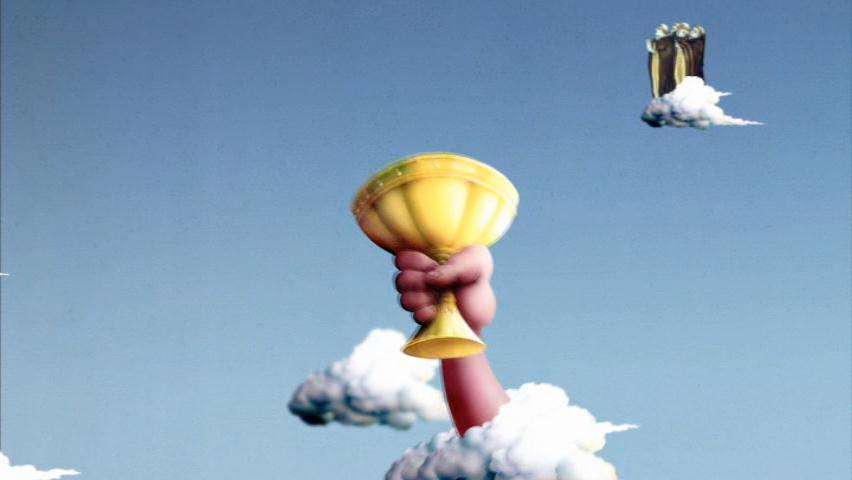
\includegraphics[width=0.8\textwidth]{grail.jpg}
%   \caption[Voorbeeld figuur.]{\label{fig:grail}Voorbeeld van invoegen van een figuur. Zorg altijd voor een uitgebreid bijschrift dat de figuur volledig beschrijft zonder in de tekst te moeten gaan zoeken. Vergeet ook je bronvermelding niet!}
% \end{figure}

% \begin{listing}
%   \begin{minted}{python}
%     import pandas as pd
%     import seaborn as sns

%     penguins = sns.load_dataset('penguins')
%     sns.relplot(data=penguins, x="flipper_length_mm", y="bill_length_mm", hue="species")
%   \end{minted}
%   \caption[Voorbeeld codefragment]{Voorbeeld van het invoegen van een codefragment.}
% \end{listing}

% \lipsum[7-20]

% \begin{table}
%   \centering
%   \begin{tabular}{lcr}
%     \toprule
%     \textbf{Kolom 1} & \textbf{Kolom 2} & \textbf{Kolom 3} \\
%     $\alpha$         & $\beta$          & $\gamma$         \\
%     \midrule
%     A                & 10.230           & a                \\
%     B                & 45.678           & b                \\
%     C                & 99.987           & c                \\
%     \bottomrule
%   \end{tabular}
%   \caption[Voorbeeld tabel]{\label{tab:example}Voorbeeld van een tabel.}
% \end{table}
